%%%%%%%%%%%%%%%%%%%%%%%%%%%%%%%%%%%%%%%%%%%%%%%%%%%%%%%%%%%%%%%%%%%%%%%%%%%%%%%%
%                                                                              %
% neural networks                                                              %
%                                                                              %
% version: 2015-05-15T1451Z                                                    %
%                                                                              %
% Will Breaden Madden                                                          %
%                                                                              %
%%%%%%%%%%%%%%%%%%%%%%%%%%%%%%%%%%%%%%%%%%%%%%%%%%%%%%%%%%%%%%%%%%%%%%%%%%%%%%%%
%                                                                              %
% DESCRIPTION                                                                  %
%                                                                              %
% This program produces neural network diagrams.                               %
%                                                                              %
%%%%%%%%%%%%%%%%%%%%%%%%%%%%%%%%%%%%%%%%%%%%%%%%%%%%%%%%%%%%%%%%%%%%%%%%%%%%%%%%
%                                                                              %
% LICENCE INFORMATION                                                          %
%                                                                              %
% This program produces a document.                                            %
%                                                                              %
% copyright (C) 2015 William Breaden Madden                                    %
%                                                                              %
% This software is released under the terms of the GNU General Public License  %
% version 3 (GPLv3).                                                           %
%                                                                              %
% This program is free software: you can redistribute it and/or modify it      %
% under the terms of the GNU General Public License as published by the Free   %
% Software Foundation, either version 3 of the License, or (at your option)    %
% any later version.                                                           %
%                                                                              %
% This program is distributed in the hope that it will be useful, but WITHOUT  %
% ANY WARRANTY; without even the implied warranty of MERCHANTABILITY or        %
% FITNESS FOR A PARTICULAR PURPOSE.  See the GNU General Public License for    %
% more details.                                                                %
%                                                                              %
% For a copy of the GNU General Public License, see                            %
% <http://www.gnu.org/licenses/>.                                              %
%                                                                              %
%%%%%%%%%%%%%%%%%%%%%%%%%%%%%%%%%%%%%%%%%%%%%%%%%%%%%%%%%%%%%%%%%%%%%%%%%%%%%%%%

\documentclass{article}

% graphics
    \usepackage{pgf}
    \usepackage{tikz}
    \usepackage{pgfplots}
    \usetikzlibrary{calc}
    \usetikzlibrary{arrows, shapes}
    \usetikzlibrary{arrows, automata}
    \usetikzlibrary{positioning}
% figures
    \usepackage{subfigure}

\begin{document}

\begin{figure}
	\centering
	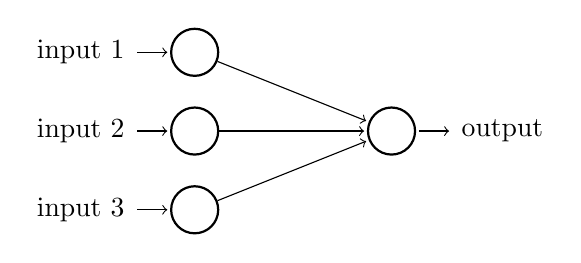
\begin{tikzpicture}[
		shorten >=1 pt,
		->,
		%draw=black!50,
		node distance=\layersep
		]
		% Define the distance between the different layers.
			\def\layersep{2.5 cm}
		\tikzstyle{every pin edge}=[
			<-,
			shorten <=1 pt
		]
		\tikzstyle{neuron}=[
			circle,
			draw,
			style=thick,
			color=black,
			%line width=1 pt,
			%fill=black!35,
			minimum size=17 pt,
			inner sep=0 pt
		]
		\tikzstyle{input neuron}=[
			neuron,
			%fill=green!50
		];
		\tikzstyle{output neuron}=[
			neuron,
			%fill=red!50
		];
		\tikzstyle{hidden neuron}=[
			neuron,
			%fill=blue!50
		];
		\tikzstyle{annot} = [
			text width=4 em,
			text centered
		]
		% Draw the input layer nodes.
			\foreach \name / \y in {1, ..., 3}
			\node[input neuron, pin=left:input \y] (I-\name) at (0,-\y) {};
		% Draw the output layer node.
			\node[output neuron, pin={[pin edge={->}]right:output}, right of=I-2] (O) {};
		% Connect every node in the hidden layer with the output layer.
			\foreach \source in {1, ..., 3}
				\path (I-\source) edge (O);
	\end{tikzpicture}
	\caption{computational element or node of artificial neural network}
	\label{figure:node_1}
\end{figure}

\begin{figure}
	\centering
	\subfigure[hard limiter]{
		\begin{tikzpicture}
			\begin{axis}[
				xtick=\empty,
				ytick={-1, 0, 1},
				xlabel=${x}$,
				ylabel=${f_{h}\left(x\right)}$,
				width=150 pt]
				\addplot+[mark=none, black]
					coordinates{
						(-1, -1)
						(0, -1)
						(0, 1)
						(1, 1)
					};
			\end{axis}
		\end{tikzpicture}
		\label{figure:hard_limiter_1}
	}
	\\
	\subfigure[threshold logic]{
		\begin{tikzpicture}
			\begin{axis}[
				ymin=-1.2,
				xtick=\empty,
				ytick={-1, 0, 1},
				xlabel=${x}$,
				ylabel=${f_{t}\left(x\right)}$,
				width=150 pt]
				\addplot+[mark=none, black]
					coordinates{
						(-1, 0)
						(0, 0)
						(1, 1)
					};
			\end{axis}
		\end{tikzpicture}
		\label{figure:threshold_logic_1}
	}
	\subfigure[sigmoid]{
		\begin{tikzpicture}
			\begin{axis}
				[
					xtick=\empty,
					ytick={-1, 0, 1},
					xlabel=${x}$,
					ylabel=${f_{s}\left(x\right)}$,
					width=150 pt
				]
				\addplot+[mark=none, smooth, black] {2/(1+e^(-x))-1};
			\end{axis}
		\end{tikzpicture}
		\label{figure:sigmoid_1}
	}
	\caption{three representative nonlinearities}
	\label{figure:three_representative_nonlinearities_1}
\end{figure}

\end{document}
